\chapter{Validated Results}
\label{cha:results}

To demonstrate the geo-based media player, we went out and did some recordings to test the functionalities we designed and implemented in this thesis. We went to “Blåa havet” in front of Kårallen, located at Linköpings University, where some students were promoting an upcoming event with some activities. We found that this was a suitable point of interest to record from different angles for our testing case. As we only had two cameras available at the time we made three sets of recordings consisting of two recordings each, with each set displaying the same scene from two different locations and angles at the same time. The desired outcomes of this test was to prove the accuracy of the relative placement algorithm and be able to swap between the recordings to view the same object at one point in time from different angles within the interface.

\section{Position Algorithm}
\label{sec:positionalgorithm}

To demonstrate the accuracy of the relative placement of geographical points in the interface, we noted the GPS-coordinates and angles at the used recording locations. We then input the coordinates into Google Maps as seen in Figure \ref{fig:googlemaps}, which is used here as a reference to prove the accuracy of our placement algorithm. We also input the same latitude, longitude and angle values into our interface to test our two algorithms when the number of objects was less then ten. Figure \ref{fig:GeomapVsGoogleBraAlg} shows the comparison between the equiretangular algorithm's placement and the real world, and Figure \ref{fig:GeomapVsGoogleDaligAlg} shows the comparison between the simplified algorithm's placement and the real world. 


\begin{figure}[ht!]
\begin{center}
	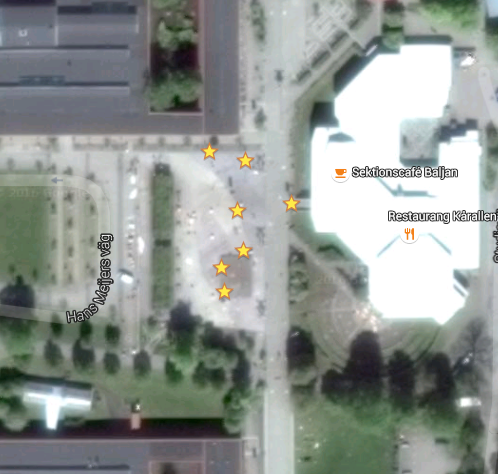
\includegraphics[scale=0.64]{Google_Maps.png}
	\caption{Google Maps view of the Streaming locations}
	\label{fig:googlemaps}
\end{center}
\end{figure}

\begin{figure}
\begin{subfigure}[b]{0.5\textwidth}
        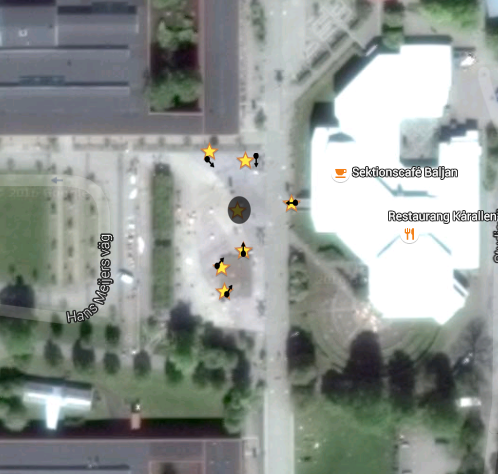
\includegraphics[width=\textwidth]{GeomapVsGoogleBraAlg.png}
        \caption{Geo-map compared to google map using equireqtangular algorithm}
        \label{fig:GeomapVsGoogleBraAlg}
    \end{subfigure}\hfill 
    \hspace{3px}
    \begin{subfigure}[b]{0.5\textwidth}
        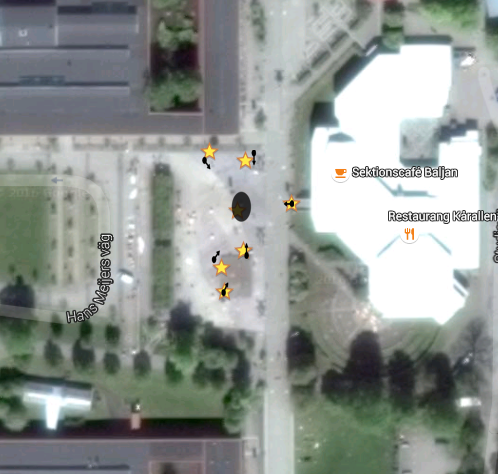
\includegraphics[width=\textwidth]{GeomapVsGoogleDaligAlg.png}
        \caption{Geo-map compared to google map using simplified algorithm}
        \label{fig:tiger}
    \label{fig:GeomapVsGoogleDaligAlg}
    \end{subfigure}
	\caption{Geo-map compared to google map with less than 10 objects}
	\label{fig:GeomapVsGoogleWithLessThan10objects}
\end{figure}

\begin{figure}
\begin{subfigure}[b]{0.5\textwidth}
       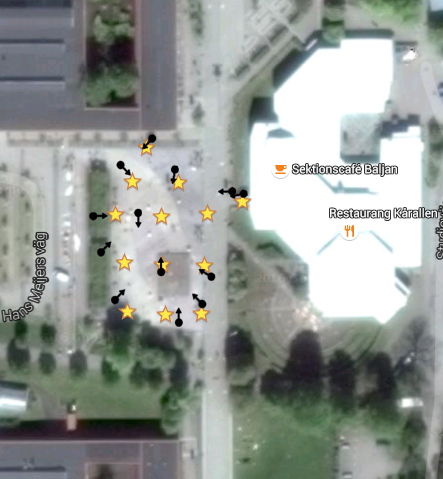
\includegraphics[width=\linewidth]{GeomapVsGoogleFleran10equi.png}
		\caption{Geo-map with more than 10 objects compared to google map using equireqtangular algorithm}
  	\label{fig:GeomapVsGoogleFleran10equi}
    \end{subfigure}\hfill 
    \hspace{3px}
    \begin{subfigure}[b]{0.5\textwidth}
       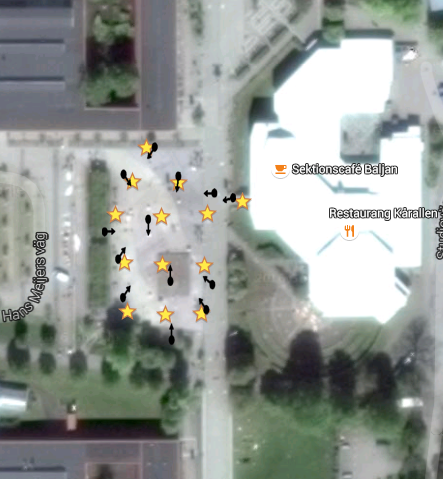
\includegraphics[width=\linewidth]{GeomapVsGoogleFleran10Dalig.png}
  \caption{Geo-map with more than 10 objects compared to google map using simplified algorithm}	\label{fig:GeomapVsGoogleFleran10Dalig}
    \end{subfigure}
	\caption{Geo-map compared to google map with more than 10 objects}
	\label{fig:GeomapVsGoogleWithMoreThan10objects}
\end{figure}

The placement of the arrow points in Figure \ref{fig:GeomapVsGoogleBraAlg} is almost an exact match to those in Figure \ref{fig:googlemaps}, at least in terms off relativity. There is a slight difference between the two and the reason for this is that the points in our geographical map is scaled to make use of the entire map, in such a way that the distance between them are increased while their relative locations between each other remain intact. When looking at the placement of arrow-points in Figure \ref{fig:GeomapVsGoogleDaligAlg},when the simplified algorithm is used, we can see that relativity is not as good but is still decent. However, when looking at Figure \ref{fig:GeomapVsGoogleFleran10equi} and \ref{fig:GeomapVsGoogleFleran10Dalig}, when there are more than ten objects, we can see that relativity when using the simplified algorithm is slightly better than the equiretangular algorithm even though both of their relativity and accuracy still is not perfect. 

This would prove the accuracy of our relative placement of the geographical points and that the equiretangular algorithm is better in terms of relativity and accuracy when the number of objects is less than ten, and that the simplified algorithm is slightly better when there are more than ten objects.

\section{Geo-based Streaming}
\label{sec:geobasedstreaming}

As we have mentioned before, our implementations is as shown in Figure \ref{fig:gpsinterface}, where we have a button that opens the geographical map, a circle that represents a “map” and arrows pointing in a direction that represents streamers and videos. When a video is selected the arrow is highlighted and that video is then played. In our test case, we set up two cameras at a time and did recordings of 90 seconds each. In these videos we captured many people doing various activities. There were people jumping the trampoline, using hoverboards, walking and biking around. When we input these three sets of two recordings each into our media player, we could swap between the two recordings of each set and watch these same events unfold from different positions and angles. In Figures \ref{fig:testview1A} and \ref{fig:testview2A} two different recordings are selected and they show the same event where, for example, the guy inside the red circle in the pictures are hoverboarding in front of the red shirt guy the same time of the videos. If we look at Figures \ref{fig:testview1B} and \ref{fig:testview2B} they show the geo-map interface of the views. Both interfaces shows that a different stream object is highlighted when a different view is shown. This would prove the desired functionality of where the user can display the same event from different geographical positions and angles.

\begin{figure}
\begin{subfigure}[b]{0.5\textwidth}
 	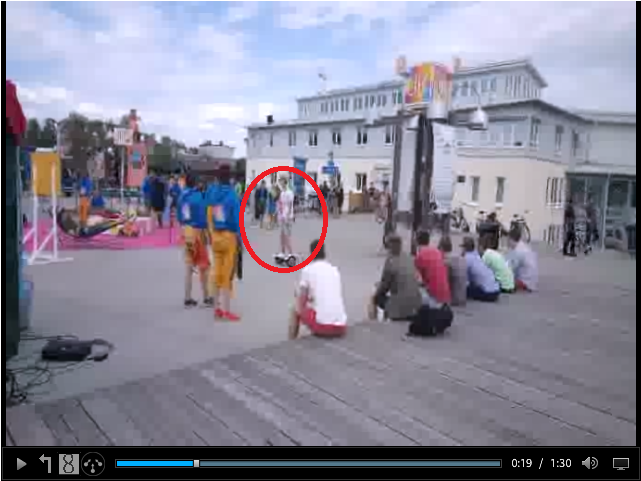
\includegraphics[width=\linewidth]{Hoverboard_1.png}
  	\caption{Test view 1 without interface showing}\label{fig:testview1A}
    \end{subfigure}\hfill 
    \hspace{3px}
    \begin{subfigure}[b]{0.5\textwidth}
	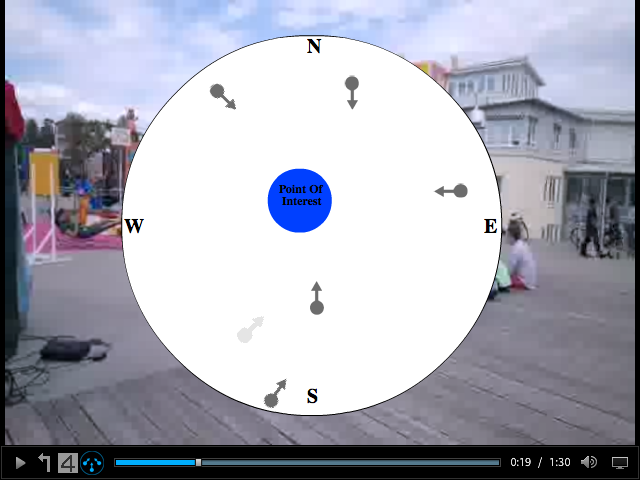
\includegraphics[width=\linewidth]{Hoverboard1medmap.png}
  	\caption{Test view 1 with interface showing}\label{fig:testview1B}
    \end{subfigure}
	\caption{Test view 1}
	\label{fig:testview1}
\end{figure}

\begin{figure}
\begin{subfigure}[b]{0.5\textwidth}
 	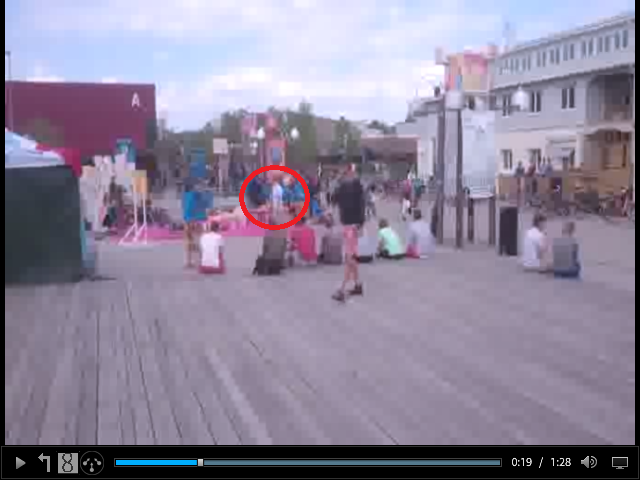
\includegraphics[width=\linewidth]{Hoverboard_2.png}
  	\caption{Test view 2 without interface showing}\label{fig:testview2A}
    \end{subfigure}\hfill 
    \hspace{3px}
    \begin{subfigure}[b]{0.5\textwidth}
	 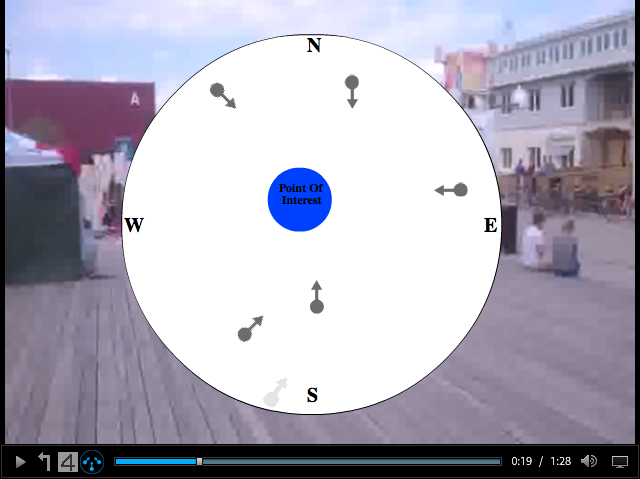
\includegraphics[width=\linewidth]{Hoverboard2medmap.png}
 	\caption{Test view 2 with interface showing}\label{fig:testview2B}
    \end{subfigure}
	\caption{Test view 2}
	\label{fig:testview2}
\end{figure}

\section{Consistency with On-demand Switching}
Even though prefetching is not implemented we can still test the consistency of the on-demand switching, looking at the time it takes to switch between different videos on-demand. The test was done by clicking between different streaming object on interface and checking the time it takes to load that view to the media player. Switching between different view was done 200 times and the time it took for each click is shown in Figure \ref{fig:clickgraph}. The graph represents the time it took to switch between each video when clicking on the streaming objects. We can see that the average time it took is roughly 140 milliseconds, or 137 milliseconds to be precise. This test is done from another computer which did not host AMS 5 which means that it had to send requests of the streams to the computer hosting the AMS 5 in order to receive the videos. Keep in mind if this consistency test were done on a different performing setup with another set of computers and connections, this result would likely vary.

%&andra värden
%Keep in mind that this test is done after the plug-in script is called which means that the average time may increase slightly. 

\begin{figure}[ht!]
\begin{center}
	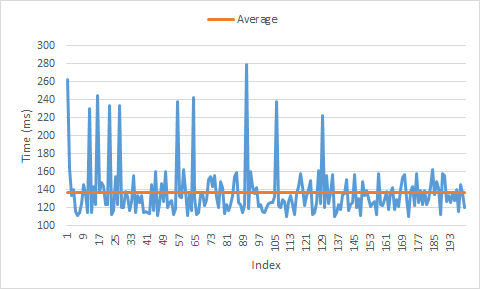
\includegraphics[scale=1]{clickgraph.png}
	\caption{Click-time interval}
	\label{fig:clickgraph}
\end{center}
\end{figure}